\section{نبود دور}
این ویژگی بیان می‌کند که شبکه‌ نباید هرگز دارای دور باشد
\cite{foerster2018survey}.
وجود دور در شبکه می‌تواند باعث مشکلاتی مانند دور زدن یک بسته در شبکه بدون رسیدن به مقصد و در نتیجه کاهش کارایی شبکه شود.
\begin{figure}
    \centering
    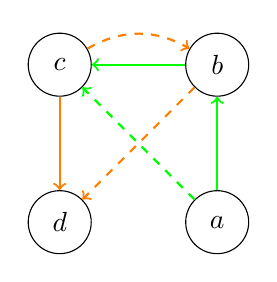
\begin{tikzpicture}[node distance={20mm},main/.style = {draw, circle,minimum size=8mm}]
        \node[main] (a)  {$a$};
        \node[main] (b) [above of=a]  {$b$};
        \node[main] (c) [left of=b] {$c$};
        \node[main] (d)  [below of=c] {$d$};
        \draw [->,green,thick] (a) -- (b);
        \draw [->,green,thick] (b) -- (c);
        \draw [->,orange,thick] (c) -- (d);
        \draw [->,green,thick,dashed] (a) -- (c);
        \draw [->,orange,thick,dashed] (c) edge[bend left] (b);
        \draw [->,orange,thick,dashed] (b) -- (d);
    \end{tikzpicture}
    \caption{ 
        شبکه‌ی ناقض ویژگی نبود دور
    }
    \label{fig:loop}
\end{figure}
به عنوان مثال شبکه‌ی رسم شده در شکل
\ref{fig:loop}
را در نظر بگیرید.
در ابتدا مسیری از
$a$
به
$d$
وجود دارد.
در این شبکه دو به روز رسانی بر روی سوییچ‌های
$a$
و
$c$
انجام می‌شود تا مسیر جدیدی از
$a$
به
$d$
ایجاد شود که اینبار ابتدا از
$c$
عبور می‌کند.
می‌توانیم از توصیف نت‌کت پویای زیر برای توصیف این شبکه استفاده کنیم:
\begin{equation*}
    \begin{aligned}
        P           & = p!1                                             \\
        Q           & = q!1                                             \\
        N           & = F \oplus p?1;N_p \oplus q?1;N_q                 \\
        N_p         & = F_p \oplus q?1;F                                \\
        N_q         & = F_q \oplus p?1;F                                \\
        SDN         & = \delta_{\mathcal{L}}(N \parallel P \parallel Q) \\
        \mathcal{L} & = \s{p!1,p?1,q!1,q?1}
    \end{aligned}
    \qquad \qquad
    \begin{aligned}
        F    = & a\ra b \oplus a\ra c \oplus a\ra d               \\
               & \oplus b\ra c \oplus b\ra d \oplus c\ra d        \\
        F_p  = & a\ra c \oplus a\ra d \oplus c\ra d               \\
        F_q  = & a\ra b \oplus a\ra c \oplus a\ra d               \\
               & \oplus b\ra c \oplus b\ra b \oplus b\ra d        \\
               & \oplus        c\ra b \oplus c\ra c \oplus c\ra d
    \end{aligned}
\end{equation*}
در توصیف بالا پردازه‌های
$P$
و
$Q$
به ترتیب وظیفه‌ای ارسال پیام برای به روز رسانی مسیر‌های سبز و نارنجی را دارند.
توجه کنید که در این توصیف پس از اجرای هر دو به روزرسانی رفتار ارسالی شبکه همانند رفتار اولیه خود می‌شود.
همانطور که در شکل
\ref{fig:loop}
مشخص است اگر به روز رسانی نارنجی پیش از به روز رسانی سبز انجام شود در شبکه یک دور شامل گره‌های
$c$
و
$b$
ایجاد می‌شود.
\begin{figure}
    \centering
    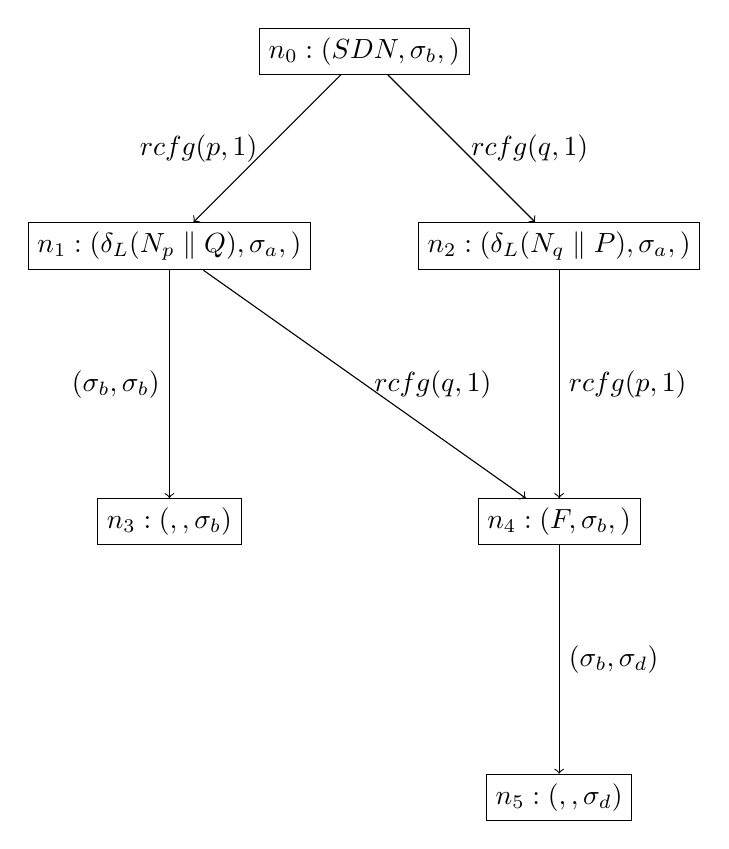
\begin{tikzpicture}[node distance={35mm},
            s/.style = {draw, rectangle,minimum width=5mm} ]
        \node[s] (n0) {$n_0: (SDN,\sigma_b,\his{})$};
        \node[s] (n1) [below left of=n0]
        {$n_1: (\delta_{\mc{L}}(N_p \parallel Q),\sigma_a,\his{})$};
        \node[s] (n3) [below of=n1]
        {$n_3: (\checkmark,\his{},\sigma_b)$};
        \node[s] (n2) [below right of=n0]
        {$n_2: (\delta_{\mc{L}}(N_q \parallel P),\sigma_a,
                \his{})$};
        \node[s] (n4) [below of=n2]
        {$n_4:(F,\sigma_b,\his)$};
        \node[s] (n5) [below of=n4]
        {$n_5:(\checkmark,\his{},\sigma_d)$};
        \draw[->] (n0) -- node[left]{$rcfg(p,1)$} (n1);
        \draw[->] (n0) -- node[right]{$rcfg(q,1)$} (n2);
        \draw[->] (n1) -- node[left]{$(\sigma_b,\sigma_b)$} (n3);
        \draw[->] (n1) -- node[right]{$rcfg(q,1)$} (n4);
        \draw[->] (n2) -- node[right]{$rcfg(p,1)$} (n4);
        \draw[->] (n4) -- node[right]{$(\sigma_b,\sigma_d)$} (n5);
    \end{tikzpicture}
    \caption{
        بخشی از سیستم انتقال 
        $SDN$
    }
    \label{fig:loop:lts}
\end{figure}
شکل
\ref{fig:loop:lts}
قسمتی از سیستم انتقال برچسب‌دار شبکه را در حالتی که یک بسته ورودی روی سوییچ
$b$
وجود داشته باشد را نشان می‌دهد.
همانطور که در شکل مشخص است پس از انجام به روز رسانی مسیر نارنجی امکان عملیاتی به شکل
$(\sigma_b,\sigma_b)$
وجود دارد که به معنی وجود حلقه در این شبکه است.
اما اگر به روز رسانی مسیر سبز هم انجام شود تنها عملیات ممکن روی بسته ارسال آن به سوییچ
$d$
است.
اکنون فرض کنید که
$\mr{E} = \sem{SDN}$
ساختمان رویداد این شبکه و
$\mc{M}$
مدل علی
$\mr{E}$
بر اساس تعریف
باشد.
در این مدل تابع متغیر
$PV$
را به صورت زیر تعریف می‌کنیم:
\begin{align*}
    \f{PV} & = \bigvee_{c \in C} c \in \mathcal{F}(ES(\vec v)) \\
    C      & = \s{c \subset E | \exists e \in c.
        l(e) = b\ra b \vee l(e) = c\ra c }
\end{align*}
در این تابع رفتار نا امن وجود پیکربندی‌ای شامل یکی از برچسب‌های
$b \ra b$
یا
$c \ra c$
در شبکه است.
همانند مثال قبل با توجه به ترتیب اجرای به‌روز‌رسانی‌ها در شبکه دو رویداد برای هر یک از عملیات‌های
$rcfg(p,1)$
و
$rcfg(q,1)$
در ساختمان رویداد وجود دارد.
فرض کنید برای رویداد‌های مرتبط با این عملیات‌ها چهار رویداد
$p_1,p_2,q_1,q_2$
وجود داشته باشد که برچسب آن‌ها به صورت زیر باشد:
\begin{align*}
    l(p_1) & = rcfg(p,1) \\
    l(p_2) & = rcfg(p,1) \\
    l(q_1) & = rcfg(q,1) \\
    l(q_2) & = rcfg(q,1)
\end{align*}
همچنین فرض کنید برچسب رویداد‌های
$bb,cc$
به ترتیب
$b\ra b,c\ra c$
باشد.
\begin{figure}
    \centering
    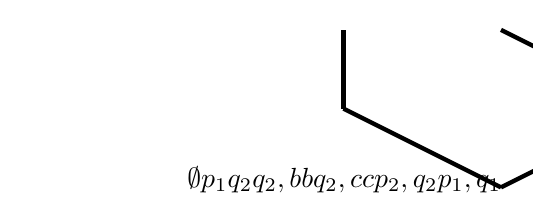
\begin{tikzpicture}
        \crd{0}{0}{$\emptyset$}
        \crd[below]{-2}{1}{$\s{p_1}$}
        \crd[below]{2}{1}{$\s{q_2}$}
        \crd[above]{2}{2}{$\s{q_2,bb}$}
        \crd[above]{4}{2}{$\s{q_2,cc}$}
        \crd[above]{0}{2}{$\s{p_2,q_2}$}
        \crd[left]{-2}{2}{$\s{p_1,q_1}$}
        \draw [ultra thick] (0,0) -- (2,1);
        \draw [ultra thick] (0,0) -- (-2,1);
        \draw [ultra thick] (2,1) -- (0,2);
        \draw [ultra thick] (2,1) -- (2,2);
        \draw [ultra thick] (2,1) -- (4,2);
        \draw [ultra thick] (-2,1) -- (-2,2);
    \end{tikzpicture}
    \caption{
        بخشی از پیکربندی‌های ساختمان رویداد 
        $SDN$
    }
    \label{fig:loop:es}
\end{figure}
شکل
\ref{fig:loop:es}
قسمتی از نمودار ساختمان رویداد این شبکه را نشان می‌دهد که در آن تمام پیکر‌بندی‌هایی وجود داشته باشد که یکی از رویداد‌های
$bb$
یا
$cc$
قابل دسترس باشد.

در این مثال می‌توان
$M_{\s{p_2},q_2}= \F$
با در نظر گرفتن
$(\e,\e,\T)$
به عنوان شاهد را یک علت واقعی وجود دور در این شبکه
معرفی کرد.
با توجه به تعریف مدل علّی در بخش
\ref{es-causal-model}
توابع متغیر‌های
$M_{\e,q_2}$
و
$EN_{\e,q_2}$
به صورت زیر تعریف می‌شوند:
\begin{align*}
    \f{M_{\e,q_2}}  & = Min(\e,q_2) \wedge Con(\e) \\
                    & = Min(\e,q_2)                \\
                    & =  \bigwedge_{q_2 \notin s'}
    \neg M_{s',q_2}                                \\
    \f{EN_{\e,q_2}} & = M_{\e,q_2}
\end{align*}
با توجه به این توابع واضح است که 
اگر مقدار
$M(\s{p_2},q_2)$
را برابر صحیح قرار دهیم آنگاه مقدار
$M(\e,q_2)$
غلط شده و در نتیجه مقدار
$EN(\e,q_2)$
هم غلط می‌شود.
برای اینکه هر کدام از مجموعه‌های شاخه‌ی راست شکل
\ref{fig:loop:es}
عضوی از مجموعه‌ی پیکربندی‌های 
$ES(\vec v)$
باشند باید داشته باشیم:
$\e \vdash q_2$
اما با توجه به این مقدار متغیر متناظر با این رابطه غلط شده است بنابراین این رابطه در 
$ES(\vec v)$
وجود ندارد، پس هیچ کدام از این مجموعه‌ها عضوی از پیکربندی‌های 
$ES(\vec v)$
نیستند.
بنابراین در این شرایط مقدار متغیر 
$PV$
غلط شده و شرط ۲.آ در تعریف 
\ref{def:extended}
برقرار می‌شود.
با توجه به گزاره‌ی 
\ref{prop:but-for}
چون
$\vec W$
در شاهد خالی است می‌توان نتیجه گرفت که
$M(\s{p_2},q_2) = \F$
علت واقعی به وجود آمدن دور در این شبکه است.
